\documentclass[10pt]{article}
\usepackage[polish]{babel}
\usepackage[utf8]{inputenc}
\usepackage[T1]{fontenc}
\usepackage{amsmath}
\usepackage{amsfonts}
\usepackage{amssymb}
\usepackage[version=4]{mhchem}
\usepackage{stmaryrd}
\usepackage{graphicx}
\usepackage[export]{adjustbox}
\graphicspath{ {./images/} }
\usepackage{bbold}

\title{XXXVI \\
 KORESPONDENCYJNY KURS Z MATEMATYKI }

\author{}
\date{}


\begin{document}
\maketitle
\section*{PRACA KONTROLNA nr 1 - POZIOM PODSTAWOWY}
październik 2006r.

\begin{enumerate}
  \item Różnica pewnej liczby trzycyfrowej i liczby otrzymanej za pomocą tych samych cyfr zapisanych w odwrotnej kolejności równa jest 495, a suma równa jest 1009. Jaka to liczba.
  \item Obliczyć $p=\frac{64^{\frac{1}{3}} \sqrt{8}+8^{\frac{1}{3}} \sqrt{64}}{\sqrt[3]{64 \sqrt{8}}}$. Znaleźć wszystkie liczby naturalne, dla których spełniona jest nierówność $x^{3}-2 x^{2}-p^{2} x+2 p^{2} \leqslant 0$.
  \item Połowę kolekcji letniej sprzedano po założonej cenie. Po obniżce ceny o $50 \%$ udało się sprzedać połowę pozostałej części towaru i dopiero kolejna $50 \%$-owa obniżka pozwoliła sklepowi pozbyć się produktu.\\
a) Ile procent zaplanowanego przychodu stanowi uzyskana ze sprzedaży kwota?\\
b) O ile procent wyjściowa cena towaru powinna była być wyższa, by sklep uzyskał zaplanowany początkowo przychód? Wyniki podać z dokładnością do 1 promila.
  \item Dach wieży kościoła ma kształt ostrosłupa, którego podstawą jest sześciokąt foremny o boku 2 m a największy z przekrojón płaszczyzną zawierającą wysokość jest trójkątem równobocznym. Obliczyć kubaturę dachu wieży kościoła. Ile 2-litrowych puszek farby antykorozyjnej trzeba kupić do pomalowania blachy, którą pokryty jest dach, jeżeli wiadomo, że 1 litr farby wystarcza do pomalowania $6 \mathrm{~m}^{2}$ blachy i trzeba uwzględnić $8 \%$ farby na ewentualne straty.
  \item Niech
\end{enumerate}

$$
f(x)=\left\{\begin{array}{rrr}
x^{2}+2 x & \text { dla } & x \leqslant 1 \\
2+\frac{1}{x} & \text { dla } & x>1
\end{array}\right.
$$

a) Narysować wykres funkcji $f$ i na jego podstawie wyznaczyć zbiór wartości funkcji.\\
b) Obliczyć $f(\sqrt{3}-1)$ oraz $f(3-\sqrt{3})$.\\
c) Rozwiązać nierówność $2 \sqrt{f(x)} \leqslant 3$ i zaznaczyć na osi $0 x$ zbiór rozwiązań.\\
6. Punkt $A=(1,0)$ jest wierzchołkiem rombu o kącie przy tym wierzchołku równym $60^{\circ}$. Wyznaczyć współrzędne pozostałych wierzchołków rombu wiedząc, że dwa z nich leżą na prostej $l: 2 x-y+3=0$. Obliczyć pole rombu. Ile rozwiązań ma to zadanie?

\section*{PRACA KONTROLNA nr 1 - POZIOM ROZSZERZONY}
\begin{enumerate}
  \item Rozwiązać nierówność $\frac{1}{\sqrt{4-x^{2}}} \geqslant \frac{1}{x-1}$ i starannie zaznaczyć zbiór rozwiązań na osi liczbowej.
  \item Rozwiązać równanie $2 \sin 2 x+2 \sin x-2 \cos x=1$. Następnie podać rozwiązania należące do przedziału $[-\pi, \pi]$.
  \item Z przystani A wyrusza z biegiem rzeki statek do przystani B, odległej od A o 140 km . Po upływie 1 godziny wyrusza za nim łódź motorowa, dopędza statek, po czym wraca do przystani A w tym samym momencie, w którym statek przybija do przystani B. Znaleźć prędkość biegu rzeki, jeżeli wiadomo, że w stojącej wodzie prędkość statku wynosi 16 km/godz, a prędkość łodzi 24 km/godz.
  \item Dane są liczby: $m=\frac{\binom{6}{4} \cdot\binom{8}{2}}{\binom{7}{3}}, n=\frac{(\sqrt{2})^{-4}\left(\frac{1}{4}\right)^{-\frac{5}{2}} \sqrt[4]{3}}{(\sqrt[4]{16})^{3} \cdot 27^{-\frac{1}{4}}}$.\\
a) Sprawdzić, wykonując odpowiednie obliczenia, że $m, n$ są liczbami naturalnymi.\\
b) Wyznaczyć $k$ tak, by liczby $m, k, n$ były odpowiednio: pierwszym, drugim i trzecim wyrazem ciągu geometrycznego.\\
c) Wyznaczyć sumę wszystkich wyrazów nieskończonego ciągu geometrycznego, którego pierwszymi trzema wyrazami są $m, k, n$. Ile wyrazów tego ciągu należy wziąć, by ich suma przekroczyła $95 \%$ sumy wszystkich wyrazów?
  \item Z wierzchołka $A$ kwadratu $A B C D$ o boku $a$ poprowadzono dwie proste, które dzielą kąt przy tym wierzchołku na trzy równe części i przecinają boki kwadratu w punktach $K$ i L. Wyznaczyć długości odcinków, na jakie te proste dzielą przekątną kwadratu. Znaleźć promień okręgu wpisanego w deltoid $A K C L$.
  \item Podstawą pryzmy przedstawionej na rysunku poniżej jest prostokąt $A B C D$,\\
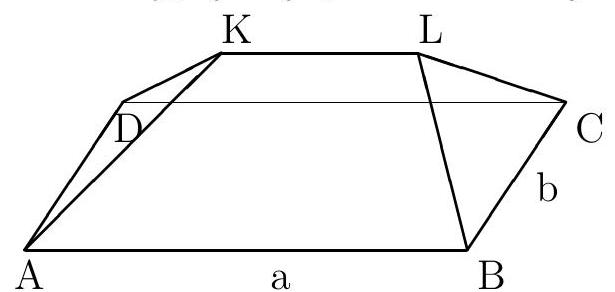
\includegraphics[max width=\textwidth, center]{2024_11_16_55121a588b067d1ba139g-02}\\
którego bok $A B$ ma długość $a$, a bok $B C$ długość $b$, gdzie $a>b$. Wszystkie ściany boczne pryzmy są nachylone pod kątem $\alpha$ do płaszczyzny podstawy. Obliczyć objętość tej pryzmy.
  \item Liczba dwuelementowych podzbiorów zbioru $A$ jest 7 razy większa niż liczba dwuelementowych podzbiorów zbioru $B$. Liczba dwuelementowych podzbiorów zbioru $A$ nie zawierających ustalonego elementu $a \in A$ jest 5 razy większa niż liczba dwuelementowych podzbiorów zbioru $B$. Ile elementów ma każdy z tych zbiorów? Ile każdy z tych zbiorów ma podzbiorów trzyelementowych?
  \item Niech $A=\left\{x \in \mathbb{R}: \frac{1}{x^{2}+23} \geqslant \frac{1}{10 x}\right\}$ oraz $B=\left\{x \in \mathbb{R}:|x-2|<\frac{7}{2}\right\}$. Zbiory $A, B, A \cup B$, $A \cap B, A \backslash B$ i $B \backslash A$ zapisać w postaci przedziałów liczbowych i zaznaczyć je na osi liczbowej.
  \item Stosując wzory skróconego mnożenia sprowadzić do najprostszej postaci wyrażenie
\end{enumerate}

$$
W=2\left(\sin ^{6} \alpha+\cos ^{6} \alpha\right)-\left(\sin ^{4} \alpha+\cos ^{4} \alpha\right)
$$

Wykorzystując wzór $\cos 2 \alpha=\cos ^{2} \alpha-\sin ^{2} \alpha$ obliczyć, dla jakich wartości kąta $\alpha$ wyrażenie $W$ przyjmuje wartość $\frac{1}{2}$.\\
4. Wiadomo, że liczby $-1,3$ są pierwiastkami wielomianu $W(x)=x^{4}-a x^{3}-4 x^{2}+b x+3$. Wyznaczyć $a, b$ i rozwiązać nierówność $\sqrt{W(x)} \leqslant x^{2}-x$.\\
5. Na kole o promieniu $r$ opisano trapez równoramienny, w którym stosunek długości podstaw wynosi $4: 3$. Obliczyć stosunek pola koła do pola trapezu oraz cosinus kąta ostrego w tym trapezie.\\
6. W ostrosłupie prawidłowym czworokątnym wszystkie krawędzie są równe $a$. Obliczyć objętość tego ostrosłupa. Znaleźć cosinus kąta nachylenia ściany bocznej do podstawy oraz cosinus kąta między ścianami bocznymi tego ostrosłupa.

\section*{PRACA KONTROLNA nr 2 - POZIOM ROZSZERZONY}
\begin{enumerate}
  \item Trzeci składnik rozwinięcia dwumianu $\left(\sqrt[3]{x}+\frac{1}{\sqrt{x}}\right)^{n}$ ma współczynnik równy 45 . Wyznaczyć wszystkie składniki tego rozwinięcia, w których $x$ występuje w potędze o wykładniku całkowitym.
  \item Niech $A=\{(x, y): y \geqslant||x-2|-1|\}, B=\left\{(x, y): y+\sqrt{4 x-x^{2}-3} \leqslant 2\right\}$. Narysować na płaszczyźnie zbiór $A \cap B$ i obliczyć jego pole.
  \item Niech $a_{n}=\frac{1+k n}{5+k^{2} n}$.\\
a) Określić monotoniczność ciągu $\left(a_{n}\right)$ w zależności od parametru $k$.\\
b) Niech $S(k)$ oznacza sumę nieskończonego ciągu geometrycznego o pierwszym wyrazie $a_{1}=1$ i ilorazie $q_{k}=\lim _{n \rightarrow \infty} a_{n}$. Sporządzić wykres funkcji $S(k)$ i na tej podstawie wyznaczyć zbiór jej wartości.
  \item Dana jest funkcja $f(x)=\cos x$. Wyznaczyć dziedzinę oraz zbiór wartości funkcji
\end{enumerate}

$$
g(x)=\sqrt{f\left(\frac{\pi}{2}-x\right)+\sqrt{3} f(x)-1}
$$

\begin{enumerate}
  \setcounter{enumi}{4}
  \item Czworokąt wypukły $A B C D$, w którym $A B=1, B C=2, C D=4, D A=3$ jest wpisany w okrąg. Obliczyć promień $R$ tego okręgu. Sprawdzić, czy w czworokąt ten można wpisać okrąg. Jeżeli tak, to obliczyć promień $r$ tego okręgu.
  \item Płaszczyzna przechodząca przez jeden z wierzchołków czworościanu foremnego i równoległa do jednej z jego krawędzi dzieli ten czworościan na dwie bryły o takiej samej objętości. Wyznaczyć pole przekroju oraz cosinus kąta nachylenia tego przekroju do płaszczyzny podstawy.
  \item Z talii 24 kart wylosowano dwie. Jakie jest prawdopodobieństwo, że obie są koloru czerwonego lub obie są figurami?
  \item Panowie X i Y założyli jednocześnie firmy i w pierwszym miesiącu działalności każda z nich miała obrot równy 50000 złotych. Po pięciu miesiącach okazało się, że obrót firmy pana X rósł z miesiąca na miesiąc o tę samą kwotę, a obrót firmy pana Y rósł co miesiąc w postępie geometrycznym. Stwierdzili również, że w drugim i trzecim miesiącu działalności firma pana X miała obrót większy od obrotu firmy pana Y o 2000 zł.\\
a) Jakie były obroty każdej z firm w pięciu początkowych miesiącach ?\\
b) Która z firm miała większą sumę obrotów w pierwszych pięciu miesiącach i o ile?\\
c) Po ilu miesiącach obrót jednej z firm (której?) przekroczy dwukrotnie obrót drugiej firmy?
  \item Tangens kąta ostrego $\alpha$ równy jest $\frac{a}{b}$, gdzie
\end{enumerate}

$$
a=(\sqrt{2+\sqrt{3}}-\sqrt{2-\sqrt{3}})^{2}, \quad b=(\sqrt{\sqrt{2}+1}-\sqrt{\sqrt{2}-1})^{2} .
$$

Wyznaczyć wartości pozostałych funkcji trygonometrycznych tego kąta. Wykorzystując wzór $\sin 2 \alpha=2 \sin \alpha \cos \alpha$, obliczyć miarę kąta $\alpha$.\\
4. Narysować wykres funkcji $f(x)=|2 x-4|-\sqrt{x^{2}+4 x+4}$. Dla jakiego $m$ pole trójkąta ograniczonego wykresem funkcji $f$ oraz prostą $y=m$ równe jest 6 ?\\
5. Harcerze rozbili 2 namioty, jeden w odległości 5 m , drugi - 17 m od prostoliniowego brzegu rzeki. Odległość między namiotami równa jest 13 m . W którym miejscu na samym brzegu rzeki (licząc od punktu brzegu będącego rzutem prostopadłym punktu położenia pierwszego namiotu) powinni umieścić maszt z flagą zastępu, by odległość od masztu do każdego z namiotów była taka sama?\\
6. Wysokość ostrosłupa trójkątnego prawidłowego wynosi $h$, a kąt między wysokościami ścian bocznych poprowadzonymi z wierzchołka ostrosłupa jest równy $2 \alpha$. Obliczyć pole powierzchni bocznej i objętość tego ostrosłupa.

\section*{PRACA KONTROLNA nr 3 - POZIOM ROZSZERZONY}
\begin{enumerate}
  \item Dla jakich wartości rzeczywistego parametru $p$ równanie $(p-2) x^{2}-(p+1) x-p=0$ ma dwa różne pierwiastki: a) ujemne? b) będące sinusem i cosinusem tego samego kąta?
  \item Jakie powinny być wymiary puszki w kształcie walca o pojemności jednego litra, by jej pole powierzchni całkowitej było najmniejsze?
  \item Z badań statystycznych wynika,że $5 \%$ mężczyzn i $0,2 \%$ kobiet to daltoniści. Wiadomo, że $55 \%$ mieszkańców Wrocławia stanowią kobiety. Jakie jest prawdopodobieństwo, że wśród 3 losowo wybranych osób przynajmniej dwie nie odróżniają kolorów?
  \item Rozwiązać nierówność $\log _{x} \frac{2-7 x}{2 x-7} \geqslant a$, gdzie $a$ jest granicą ciągu o wyrazach $a_{n}=\frac{4 n\left(\sqrt{n^{2}+n}-n\right)}{n+1}$.
  \item Pary liczb spełniające układ równań
\end{enumerate}

$$
\left\{\begin{array}{r}
-4 x^{2}+y^{2}+2 y+1=0 \\
-x^{2}+y+4=0
\end{array}\right.
$$

są współrzędnymi wierzchołków czworokąta wypukłego $A B C D$.\\
a) Wykazać, że czworokąt $A B C D$ jest trapezem równoramiennym.\\
b) Wyznaczyć równanie okręgu opisanego na czworokącie $A B C D$.\\
6. Piramida utworzona z pięciu kul, z których cztery mają taki sam promień, jest wpisana w walec. Przekrój osiowy walca jest kwadratem o boku $d$. Wyznaczyć promienie tych kul.

\begin{enumerate}
  \item Dwóch robotników może razem wykonać pewną pracę w ciągu 7 dni pod warunkiem, że pierwszy z nich rozpocznie pracę o półtora dnia wcześniej Gdyby każdy z nich pracował oddzielnie, to drugi wykonałby całą pracę o 3 dni wcześniej od pierwszego. Ile dni potrzebuje każdy z robotników na wykonanie całej pracy?
  \item Narysować na płaszczyźnie zbiór $\left\{(x, y): \sqrt{x-1}+x \leqslant 2,0 \leqslant y^{3} \leqslant \sqrt{5}-2\right\}$ i obliczyć jego pole. Wsk. Obliczyć $a=\left(\frac{\sqrt{5}-1}{2}\right)^{3}$.
  \item Obliczyć $a=\operatorname{tg} \alpha$, jeżeli $\sin \alpha-\cos \alpha=\frac{1}{5}$ i kąt $\alpha$ spełnia nierówność $\frac{\pi}{4}<\alpha<\frac{\pi}{2}$. Wyznaczyć wysokość trójkąta prostokątnego, w którym tangens jednego z kątów ostrych jest równy $a$ a pole koła opisanego na tym trójkącie wynosi $25 \pi$.
  \item Kopuła Bazyliki Św. Piotra w Watykanie ma kształt półsfery o promieniu 28 m . Przed rozpoczęciem prac renowacyjnych, na centralnie ustawionym rusztowaniu, umocowano poziomą platformę w kształcie koła. Największa odległość tej platformy od sklepienia równa jest $2,5 \mathrm{~m}$. a najmniejsza $1,5 \mathrm{~m}$. Jaka jest powierzchnia tej platformy?
  \item Trójmian kwadratowy $f(x)=a x^{2}+b x+c$ przyjmuje najmniejszą wartość równą -2 w punkcie $x=2$ a reszta z dzielenia tego trójmianu przez dwumian $(x-1)$ równa jest 4. Wyznaczyć współczynniki $a, b, c$. Narysować staranny wykres funkcji $g(x)=f(|x|)$ i wyznaczyć najmniejszą i największą wartość tej funkcji na przedziale[-1,3].
  \item Pani Zosia odcięła z kwadratowego kawałka materiału o boku 1 m wszystkie cztery narożniki i otrzymała serwetę w kształcie ośmiokąta foremnego. Postanowiła wykończyć ją szydełkową koronką o szerokości 5 cm .\\
a) Obliczyć długość boku serwety przed i po jej wykończeniu.\\
b) Wiedząc, że na zrobienie 100 centymetrów kwadratowych koronki potrzebny jest jeden motek kordonku obliczyć, ile motków musi kupić Pani Zosia, jeżeli powinna uwzględnić $2 \%$ straty materiału podczas pracy.
\end{enumerate}

\section*{PRACA KONTROLNA nr 4 - POZIOM ROZSZERZONY}
\begin{enumerate}
  \item Do zbiornika poprowadzono trzy rury. Pierwsza rura potrzebuje do napełnienia zbiornika o 4 godziny więcej niż druga, a trzecia napełnia cały zbiornik w czasie dwa razy krótszym niż pierwsza. W jakim czasie napełnia zbiornik każda z rur, jeżeli wiadomo, że wszystkie trzy rury otwarte jednocześnie napełniają zbiornik w ciągu 2 godzin i 40 minut?
  \item Stosując zasadę indukcji matematycznej wykazać prawdziwość następującego wzoru dla wszystkich $n \geqslant 1$
\end{enumerate}

$$
\frac{1^{2}}{1 \cdot 3}+\frac{2^{2}}{3 \cdot 5}+\frac{3^{2}}{5 \cdot 7}+\ldots+\frac{n^{2}}{(2 n-1) \cdot(2 n+1)}=\frac{n(n+1)}{2(2 n+1)}
$$

\begin{enumerate}
  \setcounter{enumi}{2}
  \item Nie wykorzystując metod rachunku różniczkowego wyznaczyć przedziały zawarte w $[0,2 \pi]$, na których funkcja
\end{enumerate}

$$
f(x)=\cos x+2 \cos ^{2} x+4 \cos ^{3} x+8 \cos ^{4} x+\ldots
$$

jest rosnąca.\\
4. Narysować zbiór $\left\{(x, y):|x|+|y| \leqslant 6,|y| \leqslant 2^{|x|},|y| \geqslant \log _{2}|x|\right\}$ i napisać równania jego osi symetrii. Podać odpowiednie uzasadnienie.\\
5. Pole przekroju ostrosłupa prawidłowego czworokątnego płaszczyzną przechodzącą przez przekątną podstawy i wierzchołek ostrosłupa jest trójkątem równobocznym o polu $S$. Wyznaczyć stosunek promienia kuli wpisanej w ten ostrosłup do promienia kuli opisanej na tym ostrosłupie.\\
6. Punkt $A(1,2)$ jest wierzchołkiem trójkąta równobocznego. Wyznaczyć dwa pozostałe wierzchołki tego trójkąta wiedząc, że jeden z nich leży na prostej $x-y-1=0$, a jeden z boków jest równoległy do wektora $\vec{v}=[-1,2]$. Obliczyć pole tego trójkąta. Ile jest trójkątów spełniających warunki zadania?

\begin{enumerate}
  \item Bolek i Lolek z okazji swoich 9 i 11 urodzin otrzymali od babci 200 zł do podziału. Umówili się, że starszy otrzyma większą sumę, ale nie więcej niż o połowę od otrzymanej przez brata, a ponadto średnia geometryczna obu kwot nie przekroczy iloczynu ich lat życia. Jaką maksymalną i minimalną kwotę może otrzymać starszy brat.
  \item Rozważmy zbiór wszystkich ciągów binarnych o długości 7. Wylosowano jeden ciąg.\\
a) Jakie jest prawdopodobieństwo, że będzie zawierał co najmniej 3 jedynki.\\
b) Jakie jest prawdopodobieństwo, że w tym ciągu wystąpi seria samych zer lub samych jedynek o długości co najmniej 4.
  \item W trójkącie $A B C$ dane są $\angle C A B=\frac{\pi}{3}$, wysokość $|C D|=h=5$ oraz $|B D|=d=\sqrt{2}$. Obliczyć promień okręgu wpisanego w ten trójkąt.
  \item Na jednym rysunku przedstawić staranne wykresy funkcji $f(x)=\left|\sin \left(x-\frac{\pi}{9}\right)\right|$ oraz $g(x)=-\cos \left(x+\frac{5 \pi}{18}\right)$ na przedziale $I=[-\pi, 2 \pi]$.\\
a) Odczytać z wykresu kąt $x_{0}$ taki, że $g(x)=\sin \left(x-x_{0}\right)$.\\
b) Korzystając z wykresu oraz punktu a) wyznaczyć wszystkie kąty $x \in I$, dla których $f(x)=g(x)$ oraz przedziały, dla których $g(x)>f(x)$.
  \item Na walcu o wysokości 6 cm i średnicy podstawy 16 cm opisano stożek o kącie rozwarcia $2 \alpha$ tak, że podstawa walca leży na podstawie stożka, przy czym $\operatorname{tg} \alpha=\frac{4}{3}$. Wyznaczyć minimalne wymiary prostokąta (z zaokrągleniem w górę do pełnych cm), w którym można zmieścić rozciętą powierzchnię boczną stożka i obliczyć jaki procent pola tego prostokąta stanowi powierzchnia boczna stożka.
  \item Dane są proste $k: 2 x-3 y+6=0$ oraz $l: 2 x+4 y-7=0$. Na prostej $k$ znaleźć punkt, którego obraz symetryczny względem prostej $l$ leży na osi Oy. Sporządzić rysunek.
\end{enumerate}

\section*{PRACA KONTROLNA nr 5 - POZIOM ROZSZERZONY}
\begin{enumerate}
  \item Stosując zasadę indukcji matematycznej wykazać, że liczba $7^{n}-(-3)^{n}$ jest podzielna przez 10 dla każdego naturalnego $n$.
  \item Rozwiązać nierówność $4 \log _{16} \cos 2 x+2 \log _{4} \sin x+\log _{2} \cos x+3<0$ dla $x \in\left(0, \frac{\pi}{4}\right)$.
  \item Różnica ciągu arytmetycznego $\left(a_{n}\right)$ jest liczbą mniejszą od 1. Wyznaczyć najmniejszą wartość wyrażenia $\frac{a_{1} a_{49}}{a_{50}}$, wiedząc, że $a_{51}=1$.
  \item Cięciwa paraboli o równaniu $y=-a^{2} x^{2}+5 a x-4$ jest styczna do krzywej $y=\frac{1}{-x+1}$ w punkcie o odciętej $x_{o}=2$, który dzieli tę cięciwę na połowy. Wyznaczyć parametr $a$. Podać ilustrację graficzną rozwiązania zadania.
  \item Dana jest funkcja $f(x)=\frac{2 x^{2}}{(2-x)^{2}}$.\\
a) Zbadać przebieg zmienności funkcji $f$ i naszkicować jej wykres.\\
b) Sporządzić wykres funkcji $k=g(m)$, gdzie $k$ jest liczbą rozwiązań równania
\end{enumerate}

$$
\frac{2 x^{2}}{(2-|x|)^{2}}=m
$$

w zależności od parametru rzeczywistego $m$.\\
6. W kulę o promieniu $R$ wpisano stożek, w którym tworząca jest równa średnicy podstawy. Obydwie bryły przecięto płaszczyzną równoległą do podstawy stożka. Szerokość otrzymanego w przecięciu pierścienia kołowego zawartego między powierzchnią kulistą a powierzchnią boczną stożka równa się $m$.\\
a) Znaleźć odległość płaszczyzny tnącej od wierzchołka stożka.\\
b) Przedyskutować liczbę rozwiązań w zależności od $m$ i podać interpretację geometryczną przypadków szczególnych.

\begin{enumerate}
  \item Boki trójkąta prostokątnego o polu 12 tworzą ciąg arytmetyczny. Wyznaczyć promień okręgu wpisanego w ten trójkąt.
  \item Pan Kowalski zaciągnął 31 grudnia pożyczkę 4000 złotych oprocentowaną w wysokości $18 \%$ w skali roku. Zobowiązał się spłacić ją w ciągu roku w trzech równych ratach płatnych 30 kwietnia, 30 sierpnia i 30 grudnia. Oprocentowanie pożyczki liczy się od 1 stycznia, a odsetki od kredytu naliczane są w terminach płatności rat. Obliczyć wysokość tych rat w zaokragleniu do pełnych groszy.
  \item Narysować wykres funkcji $f(x)=\left\{\begin{array}{ccc}\frac{x-1}{x} & \text { dla } & x<0, \\ \frac{1}{2} & \text { dla } & x=0, \\ \frac{x}{x+1} & \text { dla } & x>0,\end{array}\right.$ i na jego podstawie wyznaczyć:\\
a) zbiór, jaki tworzą wartości funkcji $f(x)$, gdy $x$ przebiega przedział $(-2,1)$;\\
b) zbiór rozwiązań nierówności $\frac{1}{2} \leqslant f(x) \leqslant 2$.
  \item Suma wysokości $h$ ostrosłupa prawidłowego czworokątnego i jego krawędzi bocznej $b$ równa jest 12. Dla jakiej wartości $h$ objętość tego ostrosłupa jest największa? Obliczyć pole powierzchni całkowitej ostrosłupa dla tej wartości $h$.
  \item Punkty $A(0,4)$ i $D(3,5)$ są wierzchołkami trapezu równoramiennego $A B C D$, którego podstawy $\overline{A B}$ oraz $\overline{C D}$ są prostopadłe do prostej $k$ o równaniu $x-y-2=0$. Wyznaczyć współrzędne pozostałych wierzchołków wiedząc, że wierzchołek $C$ leży na prostej $k$. Znaleźć współrzędne środka oraz promień okręgu opisanego na tym trapezie.
  \item Na kole o promieniu $r$ opisano romb. Punkty styczności są wierzchołkami czworokąta $A B C D$. Zakładając, że stosunek pola rombu do pola czworokąta równy jest $\frac{8}{3}$, obliczyć długość boku rombu i jego przekątnych. Obliczyć pole jednego z obszarów ograniczonych bokami rombu i okręgiem.
\end{enumerate}

\section*{PRACA KONTROLNA nr 6 - POZIOM ROZSZERZONY}
\begin{enumerate}
  \item Dla jakich wartości parametru $\alpha \in[0,2 \pi]$ istnieje dodatnie maksimum funkcji
\end{enumerate}

$$
f(x)=(2 \cos \alpha-1) x^{2}-2 x+\cos \alpha ?
$$

\begin{enumerate}
  \setcounter{enumi}{1}
  \item Granicą ciągu o wyrazie ogólnym $a_{n}=\frac{\sqrt{n^{4}+a n^{3}+b n}-n^{2}}{\sqrt{n^{2}+1}}$ jest większy z pierwiastków równania $4 x^{\log x}+10 x^{-\log x}=41$. Wyznaczyć parametry $a$ i $b$.
  \item Wyznaczyć równanie krzywej utworzonej przez punkty, których odległość od osi $0 x$ jest taka sama, jak odległość od półokręgu o równaniu $y=\sqrt{2 x-x^{2}}$. Sporządzić rysunek.
  \item W stożku ściętym przekątne przekroju osiowego przecinają się pod kątem prostym, a tworząca o długości $l$ nachylona jest do płaszczyzny podstawy dolnej pod kątem $\alpha$. Obliczyć pole powierzchni bocznej tego stożka ściętego oraz pole powierzchni opisanej na nim kuli.
  \item W trójkącie $\triangle A B C$ dane są podstawa $|A B|=a$, kąt ostry przy podstawie $\angle C A B=2 \alpha$ i dwusieczna tego kąta $|A D|=d$. Obliczyć pole koła opisanego na tym trójkącie. Podać warunek istnienia rozwiązania.
  \item Zbadać przebieg zmienności funkcji określonej wzorem
\end{enumerate}

$$
f(x)=\sqrt{x+1}+1+\frac{1}{\sqrt{x+1}}+\ldots
$$

gdzie prawa strona jest sumą wyrazów nieskończonego ciągu geometrycznego. Narysować jej staranny wykres.


\end{document}